\documentclass[12pt]{article}

\usepackage[utf8]{inputenc}
\usepackage{datetime}
\usepackage{amsthm}
\usepackage{amsmath}
\usepackage{amssymb}
\usepackage{enumitem}
\usepackage[english]{babel}
\usepackage{matlab-prettifier}
\usepackage{graphicx}
\usepackage[makeroom]{cancel}
\usepackage{afterpage}
\usepackage{capt-of}
\usepackage{bm}
\usepackage{float}

\DeclareMathOperator*{\argmin}{arg\,min}
\DeclareMathOperator*{\argmax}{arg\,max}

\newcommand\independent{\protect\mathpalette{\protect\independenT}{\perp}}
\def\independenT#1#2{\mathrel{\rlap{$#1#2$}\mkern2mu{#1#2}}}

\newtheoremstyle{colon}{\topsep}{\topsep}{}{}{\bfseries}{:}{ }{}
\theoremstyle{colon}
\newtheorem{exercise}{Exercise}
\newtheorem*{answer}{Answer}

\title{APC 523: Numerical Algorithms for Scientific Computing \\ Homework 1}
\author{Zachary Hervieux-Moore}

\newdate{date}{13}{03}{2019}
\date{\displaydate{date}}

\begin{document}

\maketitle

\clearpage

\begin{exercise}
  \textbf{Error in (symmetric) rounding vs. chopping}
\end{exercise}

\begin{answer}
  We will show that symmetric rounding satisfies the following bound by considering two cases:
  \begin{gather*}
    \left\lvert \frac{x - \text{rd}(x)}{x} \right\rvert  \leq 2^{-p}
  \end{gather*}

  First, we consider the case where the discarded bit is 0. For example, $x = 0.0011\textbf{01...}$ where we are rounding after the $4^{th}$ decimal point. We have
  \begin{gather*}
    x - \text{rd}(x) = \pm \left( \sum_{i=p+1}^\infty b_i 2^{-i} \right) 2^e
  \end{gather*}

  But, by assumption, $b_{p+1} = 0$, so
  \begin{gather*}
    x - \text{rd}(x) = \left( \sum_{i=p+2}^\infty b_i 2^{-i} \right) 2^e
  \end{gather*}

  Then, maximizing this expression by picking $b_i = 1$ for the remaining $b_i$'s and minimizing $x$ by picking $x = 0.1000...$ as done in class, yields the bound
  \begin{gather*}
    \left\lvert \frac{x - \text{rd}(x)}{x} \right\rvert  \leq 2^{-(p+1)} \cdot 2 = 2^{-p}
  \end{gather*}

  The second case is to consider the discarded bit is 1. For example, $x = 0.1011\textbf{10...}$, where again we are rounding after the $4^{th}$ decimal. In this case, $\text{rd}(x) = 0.1100$ as we are rounding up. Note, that this means that $x$ and $\text{rd}(x)$ will be equal, up to say decimal $j$, where $\text{rd}(x)$ will be 1 at $j$, $x$ will be 0, then $\text{rd}(x)$ will be 0 for all decimals greater than $j$ and $x$ will be 1. In the example given, $j=2$. Notice in the example, $\text{rd}(x) - x = 0.0000\textbf{01...}$, the carryover from the rounding up causes the first non zero bit to be located at decimal $p + 2$. This carryover phenomena holds in the general case. So we get
  \begin{gather*}
    \text{rd}(x) - x = \left( \sum_{i=p+2}^\infty b_i 2^{-i} \right) 2^e
  \end{gather*}

  Similar to as before, maximizing and picking the worse case for $x$ yields the bound
  \begin{gather*}
    \left\lvert \frac{\text{rd}(x)- x}{x} \right\rvert = \left\lvert \frac{x - \text{rd}(x)}{x} \right\rvert  \leq 2^{-(p+1)} \cdot 2 = 2^{-p}
  \end{gather*}
\end{answer}

\clearpage

\begin{exercise}
  \textbf{Accurate implementation of $e^x$}
\end{exercise}

\begin{answer}
  The associated tables and numbers are in the attached Jupyter notebook titled \texttt{question2.ipynb}. The written answers are here.

  \begin{enumerate}[label=\alph*)]
    \item See notebook for table of terms

    \item The value of $k$ was 18 to converge to 5 significant figures to 244.71. The relative error with the built-in function was 7.384e-5.

    \item The value of $k$ was 17 to converge to 5 significant figures to 244.69. The relative error with the built-in function was 7.897e-6. The answers did change, this method is more accurate by roughly an order of magnitude and converges faster. This is due to the fact that adding the smaller terms first can yield more accurate rounding of the smaller digits since you are rounding even smaller digits first whereas adding small numbers to a large number simply truncates them.

    \item See notebook for implementations. The method that converges the quickest with the lowest error is algorithm ii). This is the same as the positive exponent but is 3 orders of magnitude of accuracy worse because subtraction adds more error than simply adding:

      \begin{enumerate}[label=\roman*)]
        \item Left to Right: The value of $k$ was 26 to converge to 5 significant figures to 3.8363e-3. The relative error with the built-in function was 0.0613.

        \item Right to Left: The value of $k$ was 20 to converge to 5 significant figures to 4.0000e-3. The relative error with the built-in function was 0.0212. Note that this is better than the previous version which coincides with parts b) and c).

        \item Left to Right, Positive then Negative: The value of $k$ was 19 to converge to 5 significant figures to 0.0000e0. The relative error with the built-in function was 1.0. Note that this terrible performance is due to the positive and negative term canceling each other out when combined.

        \item Right to Left, Positive then Negative: The value converges to 5 significant figures to 1.0000e-2. The relative error with the built-in function was 1.447. This is the worst performance and again is caused by the cancellation of the positive and negative part with a slight mismatch due to higher precision from adding right to left.
      \end{enumerate}

    \item The simplest way is to simply invert our super accurate answer for $e$ from part c). That is $e^{-5.5} = \frac{1}{e^{5.5}}$. This yields a value of 4.0868e-3 and a relative error of 6.989e-6.
  \end{enumerate}
\end{answer}

\clearpage

\begin{exercise}
  \textbf{Error propagation in exponentiation}
\end{exercise}

\begin{answer}
  In everything that follows, I assumed that $\epsilon$ for each operation was unique.

  \begin{enumerate}[label=\alph*)]
    \item

      \begin{enumerate}[label=\roman*)]
        \item We are simply doing repeated multiplication so we get the following:
          \begin{gather*}
            x^n = x^n (1+\epsilon) \cdot \mathellipsis \cdot (1+\epsilon) = x^n (1+\epsilon)^n \\
            \approx x^n (1+n\epsilon)
          \end{gather*}

        \item This calculation is easy to do in the order of the operation:
          \begin{gather*}
            \ln(x) = \ln(x) (1+\epsilon) \\
            \implies n \ln(x) = n \ln(x) (1+\epsilon)(1+\epsilon) \\
            \approx n \ln(x) (1+2\epsilon) \\
            \implies e^{n \ln(x)} = e^{n \ln(x) (1+2\epsilon)} (1+\epsilon) \\
            \approx e^{n \ln(x)} (1 + 2 \epsilon n \ln(x))(1+\epsilon) \\
            \approx e^{n \ln(x)} (1 + 2 \epsilon n \ln(x) + \epsilon)
          \end{gather*}

      \end{enumerate}

      We would do option i) if the error is less than option ii) or:

      \begin{gather*}
      n \epsilon \leq 2 n \ln(x) \epsilon + \epsilon \\
      \implies e^{\frac{n-1}{2n}} \leq x
      \end{gather*}

    \item

      \begin{enumerate}[label=\roman*)]
        \item We have the same mechanical steps as before except that $\text{fl}(a) = a (1+\epsilon_a)$. We use the method of $x^a = e^{a \ln(x)}$.

          \begin{gather*}
            \ln(x) = \ln(x)(1+\epsilon) \\
            \implies a \ln(x) = a \ln(x) (1+\epsilon)(1+\epsilon)(1+\epsilon_a) \\
            \approx a \ln(x) (1+2\epsilon+\epsilon_a) \\
            \implies e^{a \ln(x)} = e^{a \ln(x)(1+2\epsilon+\epsilon_a)}(1+\epsilon) \\
            \approx e^{a \ln(x)} (1+2\epsilon a \ln(x) +\epsilon_a a \ln(x)+\epsilon)
          \end{gather*}

        \item This time we have $\text{fl}(x) = x (1+\epsilon_x)$ but the steps are similar.

          \begin{gather*}
            \ln(x) = \ln(x(1+\epsilon_x))(1+\epsilon) = (\ln(x) +\ln(1+\epsilon_x))(1+\epsilon)\\
            \approx (\ln(x)+\epsilon_x))(1+\epsilon) = \ln(x)(1+\epsilon)+\epsilon_x \\
            \implies a \ln(x) = a \ln(x) (1+\epsilon)(1+\epsilon) + \epsilon_x a (1+\epsilon) \\
            \approx a \ln(x) (1+2\epsilon) + a \epsilon_x \\
            \implies e^{a \ln(x)} = e^{a \ln(x)(1+2\epsilon) + a \epsilon_x}(1+\epsilon) \\
            \approx e^{a \ln(x)} (1+2\epsilon a \ln(x) + \epsilon_x a +\epsilon)
          \end{gather*}

        The problems occur when $x \approx 0$ because the logarithmic term will go to negative infinity. Or, in the second case, if $a$ is large, then we don't have the option of $\ln(x)$ canceling it out if $x \approx 1$.
      \end{enumerate}
  \end{enumerate}
\end{answer}

\clearpage

\begin{exercise}
  \textbf{Conditioning}
\end{exercise}

\begin{answer}
  We have that $f(x) = 1 - e^{-x}$.

  \begin{enumerate}[label=\alph*)]

    \item The conditioning number on $(0,1]$ is as follows:
      \begin{gather*}
        (\text{cond} f)(x) = \left\lvert \frac{x f'(x)}{f(x)} \right\rvert = \left\lvert \frac{x e^{-x}}{1 - e^{-x}} \right\rvert = \frac{x}{e^{x}-1}
      \end{gather*}

      From this, it is easy to see that $(\text{cond} f)(x) < 1$ on $(0,1]$ by using standard $e^x$ inequalities or doing the Taylor series for the denominator.
      \begin{gather*}
        (\text{cond} f)(x) = \frac{x}{x + O(x^2)} < 1
      \end{gather*}

    \item We reproduce similar steps as question 3. We also use the result of error propagation of subtraction from class. We have

      \begin{gather*}
        -x = -x(1) \\
        \implies e^{-x} = e^{-x}(1+\epsilon) \\
        \implies 1 - e^{-x} = (1-e^{-x})(1+\frac{e^{-x}}{1-e^{-x}} \epsilon) \\
        \approx (1-e^{-x})(1 + \frac{e^{-x}}{1-e^{-x}} \epsilon)
      \end{gather*}

      Thus, we make our ansatz and use standard first order approximations
      \begin{gather*}
        1-e^{-x_A} = (1-e^{-x})(1+\frac{1}{e^x-1} \epsilon) \\
        \implies \ln(1 - e^{-x_A}) = \ln(1 - e^{-x}) + \ln(1 + \frac{1}{e^x-1} \epsilon) \\
        \implies -e^{-x_A} = -e^{-x} + \frac{e^{-x}}{1-e^{-x}} \epsilon \\
        \implies -x_A = -x + \ln(1-\frac{1}{1-e^{-x}} \epsilon) \\
        \implies \left\lvert \frac{x_A - x}{x} \right\rvert = \frac{1}{x(1-e^{-x})} \epsilon = \frac{e^x}{x(e^x-1)} \epsilon
      \end{gather*}

      Thus, our condition number is
      \begin{gather*}
        (\text{cond} A)(x) = \frac{e^x}{x(e^x-1)}
      \end{gather*}

      From here, we have a monotonically decreasing function that is greater than 1 when we let $x=1$, thus it is greater than 1 for $x \in [0,1]$.

    \item The graph is attached below. (cond $A$)($x$) is very poorly conditioned near $x=0$ because the denominator of the term in front of $\epsilon_{\text{exp}}$ goes to 0 while the numerator goes to 1, this leads to an exponential rise to infinity. The root cause of this is the error introduced during the subtraction because 1 and $e^{-x}$ become very close to each other when $x$ get closer to 0.

      \begin{figure}[H]
        \centering
          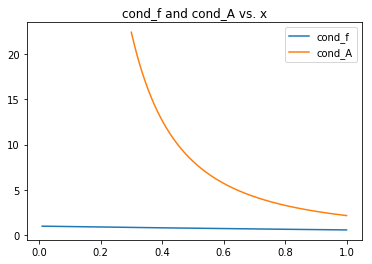
\includegraphics[width=\textwidth]{q3c.png}
        \caption{Plot of (cond $f$)($x$) and (cond $A$)($x$)}
      \end{figure}

    \item Using our previous expression from part b), we are trying to find errors that cause the $\frac{1}{e^x-1} \leq 2^b$ where $b$ is the desired bits. Solving for $x$ yields the following table.

      \begin{center}
        \begin{tabular}{ c | c }
          $b$ & $x$ \\
          \hline
          1 & $\ln(3)-\ln(2)$ \\
          2 & $\ln(5)-\ln(4)$ \\
          3 & $2\ln(9)-\ln(8)$ \\
          4 & $\ln(17)-\ln(16)$\\
        \end{tabular}
      \end{center}

    \item Now we simply plug this values into the error propagation term
      \begin{gather*}
        \frac{1}{e^x-1} \epsilon
      \end{gather*}

      Where $\epsilon = 2^{-16}$, thus we get the following
      \begin{center}
        \begin{tabular}{ c | c }
          $x$ & $error$ \\
          \hline
          $\ln(3)-\ln(2)$   & 3.051e-5 \\
          $\ln(5)-\ln(4)$   & 6.103e-5 \\
          $2\ln(9)-\ln(8)$  & 1.221e-4 \\
          $\ln(17)-\ln(16)$ & 2.441e-4 \\
        \end{tabular}
      \end{center}

    \item As part a) shows, the underlying problem is not ill-conditioned. We can hope that a better algorithm can give us more accuracy. For this, we consider the Taylor series expansion.

    \begin{gather*}
      1-e^{-x} = - \sum_{k=1}^\infty \frac{-x^k}{k!}
    \end{gather*}

    We then use Horner's method to reduce the number of multiplications:

    \begin{gather*}
      1-e^{-x} = x - \frac{x^2}{2} + \frac{x^3}{6} - \frac{x^4}{24} + O(x^5) \\
      = x \left(1+x \left(-\frac{1}{2}+x \left(\frac{1}{6}+x \left(-\frac{1}{24}+x \left(O(x^5) \right) \right) \right) \right) \right)
    \end{gather*}

  \end{enumerate}
\end{answer}

\clearpage

\begin{exercise}
  \textbf{Limits in $\mathbb{R}(p,q)$}
\end{exercise}

\begin{answer}
  The code used to accomplish this question is found in \texttt{question5.ipynb}. The answer to the questions are as follows. $n_{\text{stop}} = 10e16$ where it converged onto the value of $1.0$ for the remained of $n$. The table of intermediate values are in the notebook. The explanation for why it converges to 1 is as follows. $10^16 ~ 2^53$. As we recall, there are 52 bits in the mantissa which means when we do $1/n$ with such a large $n$, it gets rounded down to 0. Thus, we are left with $1^n$ which is of course 1.
\end{answer}

\clearpage

\begin{exercise}
  \textbf{Fun with square roots}
\end{exercise}

\begin{answer}
  Note, there are accompanying plots in the notebook \texttt{question6.ipynb}. First, we note the staircase patterns of the numbers. At iteration 54, it becomes a line at 1. Again, this is due to the mantissa having only 52 bits, so doing 54 square roots will force any floating point number to 1. At which point any power returns 1. But why the staircase pattern? If you look through my plots, you can see as we vary the number of iterations from 45 to 54, the staircase gets steeper and the steps are not evenly spaced. That is, the horizontal of the step grows logarithmically. Again, this is due to only having a fixed number of points to represent the real number continuum. Floating point numbers are distributed logarithmically to keep relative error consistent. That is, when we round, we'd prefer the relative error of rounding small numbers to be equal to rounding large numbers.

  One thing to notice is that the blue lines are always below the orange (the true) value of doing these successive square roots and squares. It may be tempting to think that some numbers get rounded up after square rooting and so the result squares should be larger than the true value. However, as square roots are irrational numbers, we calculate them using Taylor series approximations. Thus, we can always ensure that are floating point numbers match however many digits we can fit. As a result, we are always subject to truncation error which always results in an underestimate of the true value when we reapply the powers of 2.

  The final interesting thing to note is why certain is why certain values are extremely close to their true values. For example, 2.719 and 7.3891. This is because $2.719^{1/2^{52}} = 1.0000000000000002$ after rounding and $7.3891^{1/2^{52}} = 1.0000000000000004$ which are the next two smallest numbers larger than 1 in floating point numbers. To reiterate, because there is no machine number between these numbers, then every value from $2.719$ to $7.3891$ gets truncated to $1.0000000000000002$. This is why the stair case pattern is formed.
\end{answer}

\clearpage

\begin{exercise}
  \textbf{The issue with polynomial roots}
\end{exercise}

\begin{answer}
  Most of the answers associated with this question can be found in the Jupyter notebook \texttt{question7.ipynb}.

  \begin{enumerate}[label=\alph*)]
    \item The integer coefficients are listed in the first cell of the notebook.

    \item Code in the notebook. The Netwon-Raphson method returns 19.999995 with an initial guess of 21. I would classify this as convergent. However, Numpy's built in \texttt{roots()} function return 20.00054 which is different by a non trivial amount. It is also worse than the other method.

    \item Code in the notebook. For $\delta = 10^{-8}$, it converges to 9.585. For $\delta = 10^{-6}$, it converges to 7.752. For $\delta = 10^{-4}$, it converges to 5.969. For $\delta = 10^{-2}$, it converges to 5.470. These are clearly huge deviations from 20 even though the pertubations are small.

    \item Code in the notebook. With this change, roots 16 and 17 disappear completely and become complex. In fact, 10 out of the 20 roots become complex with a pertubation of $\delta = 2^{-23}$.

    \item To find the conditioning number, we first not that a deviation in $a_i$ of $\delta_{a_i}$ will yield a deviation in $\Omega_k$ of $\delta_{\Omega_k}$ that satisfies the following
      \begin{gather*}
        p_{a_i + \delta_{a_i}}(\Omega_k + \delta_{\Omega_k}) = 0
      \end{gather*}

      Where $p_{a_i + \delta_{a_i}}$ denotes the shifted polynomial. We write out this complete polynomial
      \begin{gather*}
        p_{a_i + \delta_{a_i}}(\Omega_k + \delta_{\Omega_k}) = a_0 + a_1(\Omega_k + \delta_{\Omega_k}) + \mathellipsis \\
        + (a_i + \delta_{a_i})(\Omega_k + \delta_{\Omega_k})^i + \mathellipsis + (\Omega_k + \delta_{\Omega_k})^n
      \end{gather*}

      Which we simplify and do a first order approximation on
      \begin{gather*}
        = a_0 + a_1 \Omega_k (1 + \frac{\delta_{\Omega_k}}{\Omega_k}) + \mathellipsis + (a_i + \delta_{a_i})\Omega_k^i (1 + i\frac{\delta_{\Omega_k}}{\Omega_k}) + \mathellipsis + \Omega_k^n (1 + n \frac{\delta_{\Omega_k}}{\Omega_k })
      \end{gather*}

      Now we rearrange this into a different form for clarity
      \begin{align*}
        = a_0 &+ a_1 (\Omega_k + \Omega_k \delta_{\Omega_k}) \\
        &+ a_2 (\Omega_k^2 + 2 \Omega_k \delta_{\Omega_k}) \\
        &+ a_3 (\Omega_k^3 + 3 \Omega_k^2 \delta_{\Omega_k}) \\
        &+ \mathellipsis \\
        &+ (a_i + \delta_{a_i})(\Omega_k^i + i \Omega_k^{i-1} \delta_{\Omega_k}) \\
        &+ \mathellipsis \\
        &+ (\Omega_k^n + n \Omega_k^{n-1} \delta_{\Omega_k})
      \end{align*}

      Which, we notice that all the terms infront of $\delta_{\Omega_k}$ is precisely $p'(\Omega_k$. Thus we have that
      \begin{gather*}
        \delta_{a_i} \Omega_k^i + p'(\Omega_k) \delta_{\Omega_k} = 0 \\
        \implies \frac{\partial \Omega_k}{\partial a_i} = -\frac{\Omega_k^i}{p'(\Omega_k)}
      \end{gather*}

      So we conclude that the conditioning for the $a_i$ is
      \begin{gather*}
        (\text{cond} \Omega_k)(a_i) = \left\lvert \frac{a_i \frac{\partial \Omega_k}{\partial a_i}}{\Omega_k} \right\rvert = \left\rvert \frac{a_i \Omega_k^i}{\Omega_k p'(\Omega_k)} \right\rvert
      \end{gather*}

      Which of course is only part of the total condition and so our answer is

      \begin{enumerate}[label=\roman*)]
        \item
          \begin{gather*}
            (\text{cond} \Omega_k)(\overrightarrow{a}) = \frac{1}{\lvert \Omega_k p'(\Omega_k) \rvert} \sum_i \lvert a_i \Omega_k^i \rvert
          \end{gather*}

        \item Code in the notebook. But the resulting condition numbers are:
          \begin{gather*}
            (\text{cond} \Omega_{14})(\overrightarrow{a}) = 7.193916e+13 \\
            (\text{cond} \Omega_{16})(\overrightarrow{a}) = 3.044400e+13 \\
            (\text{cond} \Omega_{17})(\overrightarrow{a}) = 2.593885e+13 \\
            (\text{cond} \Omega_{20})(\overrightarrow{a}) = 1.373204e+11
          \end{gather*}

        \item The condition number is incredibly high, so any small change in the inputs will cause huge changes to the outputs. This makes a sufficiently clever algorithm non-existent.
      \end{enumerate}
  \end{enumerate}
\end{answer}

\clearpage

\begin{exercise}
  \textbf{Recurrence in reverse}
\end{exercise}

\begin{answer}
  \

  \begin{enumerate}[label=\alph*)]
    \item The first reversal is
      \begin{gather*}
        y_k = \frac{e}{k+1} - \frac{1}{k+1}y_{k+1}
      \end{gather*}

      Expanding these yields,
      \begin{align*}
        y_k &= \frac{e}{k+1} - \frac{1}{k+1}(\frac{e}{k+2} - \frac{1}{k+2}y_{k+2} ) \\
        &= \frac{e}{k+1} - \frac{e}{(k+1)(k+2)} + \frac{1}{(k+1)(k+2)}y_{k+2} ) \\
        &\ \vdots \\
        &= e \sum_{j=1}^{N-k} \frac{(-1)^{j+1}}{\prod_{i=1}^j (k+i)} + (-1)^{N-k} \frac{y_N}{\prod_{i=1}^{N-k} (k+i)}
      \end{align*}

    \item We use the definition of condition,
      \begin{gather*}
        (\text{cond} g_k)(y_N) = \left\lvert \frac{g_k' y_N}{y_k} \right\rvert = g_k' \left\lvert \frac{y_N}{y_k} \right\rvert
      \end{gather*}

      The sequence is monotonic so we know that $\left\lvert \frac{y_N}{y_k} \right\rvert \leq 1$. ee also sub in the derivative of $g_k$ to get
      \begin{gather*}
        (\text{cond} g_k)(y_N) = \frac{1}{\prod_{i=1}^{N-k} (k+i)} = \frac{k!}{N!}
      \end{gather*}

      Now, we know that the condition number relates the input error and output error as follows
      \begin{gather*}
        (\text{cond} g_k)(y_N) \epsilon_{y_N} = \epsilon_{y_k}
      \end{gather*}

      But, by assumption, we have $\epsilon_{y_N} = 1$, So we get
      \begin{gather*}
        \epsilon_{y_k} = \frac{k!}{N!}
      \end{gather*}

      Solving for N (using Gamma functions) will give the value of $N$ required to get the desired error.

    \item We take $\epsilon_{y_k} = 2e^{-16}$ and $k=20$, our previous part says that we need a value of $N=32$ to get the error desired.

    \item Code attached in notebook \texttt{question8.ipynb}. The value we find is within the eps of the machine when compared to Wolfram Alpha.

  \end{enumerate}
\end{answer}

\end{document}